\documentclass[tikz,border=10pt]{standalone}
\usepackage{tikz}
\usetikzlibrary{shapes, arrows.meta, positioning}
\begin{document}
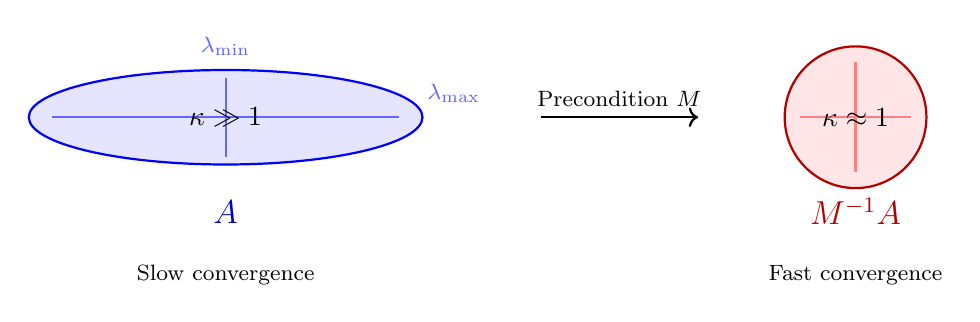
\begin{tikzpicture}
    % Original matrix visualization
    \begin{scope}
        \draw[thick, blue, fill=blue!10] (0,0) ellipse (2.5 and 0.6);
        \node[blue!80!black, font=\large] at (0,-1.2) {$A$};

        % Eigenvalue lines
        \draw[blue!60, thick] (-2.2,0) -- (2.2,0);
        \draw[blue!60, thick] (0,-0.5) -- (0,0.5);

        % Condition number indication
        \node[blue!60, font=\footnotesize] at (2.9,0.3) {$\lambda_{\max}$};
        \node[blue!60, font=\footnotesize] at (0,0.9) {$\lambda_{\min}$};

        \node at (0,0) {$\kappa \gg 1$};
    \end{scope}

    % Arrow
    \draw[->, thick] (4,0) -- (6,0) node[above,midway,font=\footnotesize]{Precondition $M$};

    % Preconditioned matrix visualization
    \begin{scope}[shift={(8,0)}]
        \draw[thick, red!70!black, fill=red!10] (0,0) circle (0.9);
        \node[red!70!black, font=\large] at (0,-1.2) {$M^{-1}A$};

        % Eigenvalue lines (more balanced)
        \draw[red!50, thick] (-0.7,0) -- (0.7,0);
        \draw[red!50, thick] (0,-0.7) -- (0,0.7);

        \node at (0,0) {$\kappa \approx 1$};
    \end{scope}

    % Performance indicators
    \node[font=\footnotesize] at (0,-2) {Slow convergence};
    \node[font=\footnotesize] at (8,-2) {Fast convergence};
\end{tikzpicture}
\end{document}